\documentclass[11pt,a4paper]{article}
\usepackage[utf8]{inputenc}
\usepackage[margin=1in]{geometry}
\usepackage{amsmath,amssymb,amsfonts,amsthm}
\usepackage{nccmath}          % local flush-left equations (fleqn) for the RAG part
\usepackage{xcolor}
\usepackage{booktabs}
\usepackage{tcolorbox}
\usepackage{fancyhdr}
\usepackage{listings}
\usepackage{titlesec}
\usepackage{tikz}
\usetikzlibrary{shapes.geometric, shapes.misc, arrows.meta, positioning, calc}
\usepackage[hypertexnames=false]{hyperref}

% ---------------------------------------------------------------------------
% Colors (from ProblemDefinition.tex and recurring-deposit-proof.tex)
\definecolor{thickgreen}{HTML}{008000}
\definecolor{primary}{HTML}{1A365D}
\definecolor{secondary}{HTML}{2B6CB0}
\definecolor{accent}{HTML}{D69E2E}
\definecolor{bglight}{HTML}{F7FAFC}
\definecolor{darktext}{HTML}{2D3748}

% Title block in the same layout as article's \maketitle, usable repeatedly
\newcommand{\parttitle}[3]{%
  \begin{center}
    {\LARGE #1\par}\vskip 1.5em
    {\large #2\par}\vskip 1em
    {\large #3\par}
  \end{center}\par\vskip 1.5em}

% Real typewriter underscore (OT1 \_ is drawn as a thin rule).
\newcommand{\ttus}{\char95}

% Styles follow LangGraph's own Mermaid output: stadium-shaped
% __start__/__end__, rectangular nodes, dashed conditional edges and
% solid fixed edges.
\tikzset{
    terminal/.style={rounded rectangle, draw, fill=violet!15,
                     minimum height=8mm, minimum width=22mm,
                     font=\ttfamily\small},
    graphnode/.style={rectangle, rounded corners=2pt, draw, fill=blue!8,
                      minimum height=9mm, minimum width=30mm,
                      font=\ttfamily\small},
    toolnode/.style={graphnode, align=left, text width=62mm},
    fixed/.style={-{Stealth[length=2.5mm]}, thick},
    conditional/.style={-{Stealth[length=2.5mm]}, thick, dashed},
    edgelabel/.style={font=\scriptsize\ttfamily, fill=white, inner sep=1pt}
}

% \agentgraph{<tool list, one per line separated by \\>}
\newcommand{\agentgraph}[1]{%
\begin{tikzpicture}[node distance=14mm and 18mm]
    \node[terminal] (start) {\ttus{}\ttus{}start\ttus{}\ttus{}};
    \node[graphnode, below=of start] (agent) {AdminAgent};
    \node[toolnode, right=of agent] (tool)
        {\textbf{tool}\\[2pt]{\scriptsize #1}};
    \node[graphnode, below=of agent] (exit) {ExitGuardrail};
    \node[terminal, below=of exit] (end) {\ttus{}\ttus{}end\ttus{}\ttus{}};

    \draw[conditional] (start) -- node[edgelabel] {continue} (agent);
    \draw[conditional] (start.west) -- ++(-18mm,0) |- node[edgelabel, pos=0.25] {end} (end.west);
    \draw[conditional] (agent.20) -- node[edgelabel, above] {continue} (tool.west |- agent.20);
    \draw[fixed] (tool.west |- agent.-20) -- (agent.-20);
    \draw[conditional] (agent) -- node[edgelabel] {end} (exit);
    \draw[fixed] (exit) -- (end);
\end{tikzpicture}%
}

\pagestyle{plain}

\begin{document}

% ===========================================================================
% financial-formulas.tex
% ===========================================================================
\begingroup
\newgeometry{margin=1in}
\setcounter{section}{0}
\fontsize{12}{14.5}\selectfont

\parttitle{\textbf{Financial Deposit and Valuation Formulas}}{Project Documentation}{\today}

\section{Recurring Deposit Formula}
The value of a recurring deposit (derived in \texttt{recurring-deposit-proof.tex}) is calculated as follows:
\[
\text{Value} = \frac{Y_d}{T_d} \cdot I \cdot \frac{\left[ 1 - \left(1 + \frac{C_d \cdot r}{100 \cdot Y_d}\right)^{\frac{T_d}{C_d}} \right] \left(1 + \frac{C_d \cdot r}{100 \cdot Y_d}\right)^{\frac{R_d}{C_d}}}{1 - \left(1 + \frac{C_d \cdot r}{100 \cdot Y_d}\right)^{\frac{R_d}{C_d}}}
\]

\subsection*{Parameter Definitions}
\begin{itemize}
    \item $I$: Installment amount deposited at the end of every payment period $R_d$
    \item $r$: Annual rate of interest (\%)
    \item $Y_d$: Days in a year
    \item $R_d$: Days in a recurring payment period
    \item $C_d$: Compounding frequency in days
    \item $T_d$: Total tenure in days
\end{itemize}

\section{Fixed Deposit Formula}
The maturity amount $A$ for a fixed deposit is given by:
\[
A = p \left( 1 + \frac{r \cdot C_d}{100 \cdot Y_d} \right)^{\frac{T_d}{C_d}}
\]

\subsection*{Parameter Definitions}
\begin{itemize}
    \item $A$: Final maturity amount
    \item $p$: Principal amount deposited
    \item $r$: Annual rate of interest (\%)
    \item $C_d$: Compounding frequency in days
    \item $Y_d$: Days in a year
    \item $T_d$: Total tenure in days
\end{itemize}

\section{\texorpdfstring{Value at the End of $n$ Years}{Value at the End of n Years}}
The discounted present value or value at the end of $n$ years is given by:
\[
A(n) = \frac{A}{1 + \frac{n \cdot R_i}{100}}
\]

\subsection*{Parameter Definitions}
\begin{itemize}
    \item $A(n)$: Value at the end of $n$ years / time $T$
    \item $A$: Base amount
    \item $n$: Number of years
    \item $R_i$: Annual discount or interest rate (\%)
\end{itemize}

\clearpage
\endgroup

% ===========================================================================
% ProblemDefinition.tex
% ===========================================================================
\begingroup
\newgeometry{margin=1in}

\section*{Markov Decision Process / Planning Problem}

\[
\begin{aligned}
&\text{1. } s \in \mathbf{S} \quad \text{and} \quad a \in \mathbf{A} \\[6pt]
&\text{2. Initial state } s_{\text{initial}} \in \mathbf{S} \\[6pt]
&\text{3. GoalState } s_{\text{Goal}} \in \mathbf{S} \\[6pt]
&\text{4. } \forall (s, a) \in \mathbf{S} \times \mathbf{A}, \exists r \in \mathbb{R} \quad \text{and} \quad \exists s' \in \mathbf{S}: \\
&\qquad s' = \mathbf{nextState}(s, a) \quad \text{(Find out from the environment)} \\
&\qquad r = \mathbf{reward}(s, a) \quad \text{(Get from the environment)} \\[6pt]
&\text{5. Planning problem: Find } \mathbf{a}^* = (a_0, a_1, \dots, a_T) \text{ and } \mathbf{s}^* = (s_{\text{initial}}, s_1, \dots, s_T, s_{\text{Goal}}) \text{ to maximize total reward } \left(\sum_{i=0}^{T} r_i\right). \\[6pt]
&\text{6. Problem definition: Find the } \mathbf{S}, \mathbf{A}, \mathbf{nextState}, \text{and } \mathbf{reward} \text{ functions. } \\[6pt]
&\text{7. }\textcolor{thickgreen}{\textbf{AI}}\text{, Please solve this problem.}
\end{aligned}
\]

\clearpage
\endgroup

% ===========================================================================
% RagEvaluationMetrics.tex
% ===========================================================================
\begingroup
\newgeometry{margin=1in}

\parttitle{\textbf{RAG Evaluation Metrics and System Architecture}}{\textbf{System Design \& Formulations}}{\today}

\begin{fleqn}[0pt]

\section*{1. System Architecture Diagram}

Below is the schematic representation of the Retrieval-Augmented Generation (RAG) pipeline showing the query $Q$, document database $D$, retrieved contexts $(C_1, C_2, C_3)$, and generated answer $A$.

\begin{figure}[htbp]
\centering
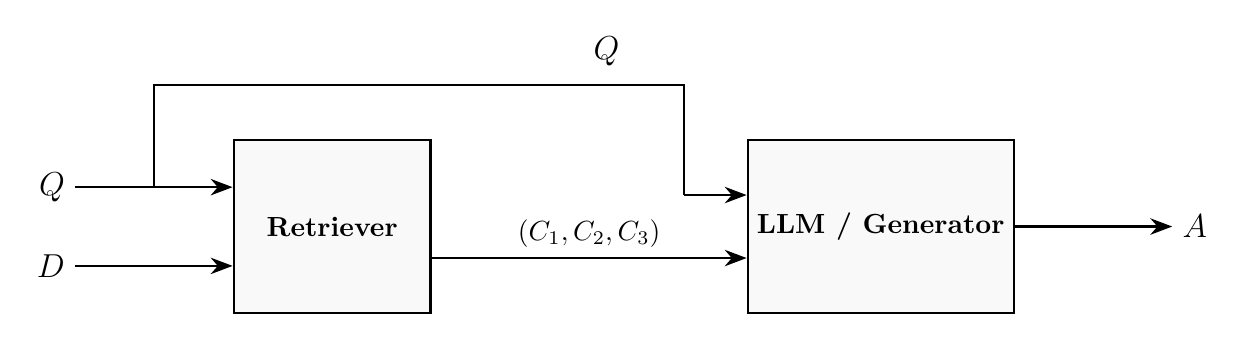
\begin{tikzpicture}[
    box/.style={draw, rectangle, minimum width=2.5cm, minimum height=2.2cm, thick, fill=gray!5, align=center},
    arrow/.style={-{Stealth[scale=1.2]}, thick}
]

    % Nodes / Blocks
    \node[box] (retriever) {\textbf{Retriever}};
    \node[box, right=4.0cm of retriever] (generator) {\textbf{LLM / Generator}};

    % Inputs on the left
    \draw[arrow] ($(retriever.west)+( -2.0, 0.5 )$) -- ($(retriever.west)+( 0, 0.5 )$) 
        node[pos=0, left] {\large $Q$};
    \draw[arrow] ($(retriever.west)+( -2.0, -0.5 )$) -- ($(retriever.west)+( 0, -0.5 )$) 
        node[pos=0, left] {\large $D$};

    % Connection between Retriever and Generator: Context (C1, C2, C3)
    \draw[arrow] ($(retriever.east)+( 0, -0.4 )$) -- ($(generator.west)+( 0, -0.4 )$) 
        node[midway, above] {$(C_1, C_2, C_3)$};

    % Tap/Feedback line sending Q directly to the second block
    \draw[thick] ($(retriever.west)+( -1.0, 0.5 )$) -- ++(0, 1.3) coordinate (topcorner) -- ($(generator.west) + ( -0.8, 1.8 )$) -- ($(generator.west) + ( -0.8, 0.4 )$);
    \draw[arrow] ($(generator.west) + ( -0.8, 0.4 )$) -- ($(generator.west) + ( 0, 0.4 )$);
    \node[above] at ($(retriever.north)!0.5!(generator.north) + (0, 0.8)$) {\large $Q$};

    % Output on the right
    \draw[arrow] (generator.east) -- ++(2.0,0) 
        node[right] {\large $A$};

\end{tikzpicture}
\caption{Retrieval-Augmented Generation (RAG) Data Flow Architecture}
\end{figure}

\vspace{0.5cm}

\section*{2. Mathematical Formulations of RAG Metrics}

\subsection*{2.1. Faithfulness}
\hspace*{1em}%
\[
\text{Faithfulness}(A, C_{1:n}) = \frac{\text{Number of claims in } A \text{ that can be inferred from the context } C_{1:n}}{\text{Total number of claims in } A}
\]

\subsection*{2.2. Context Relevance}
\hspace*{1em}%
\[
\text{ContextRelevance}(Q, C_{1:n}) = \frac{1}{n} \sum_{i=1}^{n} \left( \frac{Q \cdot C_i + 1}{2} \right) = \frac{1}{2} \left(\frac{1}{n}\left(Q \cdot \sum_{i=1}^{n} C_i\right) + 1 \right)
\]

\[
\text{ContextRelevance}(Q, C_{1:n}, \beta) = \frac{\sum\limits_{i=1}^{n} \mathbb{I}(Q \cdot C_i > \beta)}{n} \quad \text{where } \beta \text{ is the bound on the semantic similarity}
\]

\subsection*{2.3. Answer Relevance}
\hspace*{1em}%
\[
\text{AnswerRelevance}(Q, A) = \frac{1}{n} \sum_{i=1}^{n} \left( \frac{Q \cdot Q_i(A) + 1}{2} \right) = \frac{1}{2} \left(\frac{1}{n}\left(Q \cdot \sum_{i=1}^{n} Q_i(A)\right) + 1 \right)
\]

\subsection*{2.4. Context Recall}
\hspace*{1em}%
\[
\text{ContextRecall}(GT, C_{1:n}) = \frac{1}{n} \sum_{i=1}^{n} \left( \frac{GT \cdot C_i + 1}{2} \right) = \frac{1}{2} \left(\frac{1}{n}\left(GT \cdot \sum_{i=1}^{n} C_i\right) + 1 \right)
\]

\end{fleqn}

\clearpage
\endgroup

% ===========================================================================
% brute-force-goal-search.tex
% ===========================================================================
\begingroup
\newgeometry{margin=0.65in}
\setcounter{section}{0}
\titlespacing*{\section}{0pt}{8pt}{4pt}
\lstset{
    basicstyle=\ttfamily\small,
    keywordstyle=\color{blue}\bfseries,
    commentstyle=\color{gray}\itshape,
    stringstyle=\color{teal},
    frame=single,
    breaklines=true,
    captionpos=b,
    tabsize=4,
    showspaces=false,
    showstringspaces=false,
    showtabs=false,
    keepspaces=true
}

\vspace*{-0.4in}
\parttitle{\textbf{Best Goal Search Algorithm}\vspace{-0.25in}}{Typeset from Manuscript Notes}{\today}

\section{Overview \& Time Complexity}
\texttt{GoalSearch.BestSearch} navigates state transitions from an initial
state $S_0$ towards a goal state $S_g$. It is an iterative depth-first search
over an explicit stack. If $S_g$ is reached, that path is returned. Otherwise,
it returns the path to the leaf state with the highest balance among the
leaves it visits.

\begin{equation*}
\underline{\text{Best Goal Search}} \implies \text{Complexity } O\!\left(|A|^{\text{MAX-DEPTH}}\right)
\end{equation*}

\noindent
Where:
\begin{itemize}\itemsep 0pt \parskip 0pt
    \item $A = (A_0, \dots, A_{|A|-1})$: The ordered list of available actions
          (deposit schemes), indexed by $a$.
    \item $|A|$: The branching factor (number of actions).
    \item $\text{MAX-DEPTH}$: The deepest stack reached before the
          reachability test fails (bounded by the goal time horizon).
\end{itemize}

\section{Interface}
\begin{itemize}\itemsep 0pt \parskip 0pt
    \item \textbf{Transition}: $(S', c) = T(S, A_a)$ returns the successor
          state $S'$ and the number of times $c$ that action $A_a$ is
          repeated to reach it.
    \item \textbf{Reachability test}: $\mathit{isGR}(S', S_g)$ returns one of:
          \begin{itemize}\itemsep 0pt \parskip 0pt
              \item \texttt{GOAL\_REACHED}: $S'$ satisfies the goal.
              \item \texttt{GOAL\_NOT\_YET\_REACHED}: $S'$ can be extended
                    further.
              \item \texttt{GOAL\_NOT\_REACHABLE}: $S'$ overshoots the goal
                    and is discarded.
          \end{itemize}
    \item \textbf{Stack entries}: each entry is $((a, c), S')$: the action
          index, its repeat count, and the state it produced.
\end{itemize}

\clearpage
\section{Typeset Pseudocode}

% Keep the whole algorithm on one page.
\noindent
\begin{minipage}{\linewidth}
\begin{lstlisting}[language=Python, caption={Best Goal Search Pseudocode}]
GoalSearch(Sg, A, T, isGR)

BestSearch(S0):
    S = S0, stack = [], a = 0
    best = [], bestBalance = 0
    prev = GOAL_NOT_YET_REACHED

    loop:
        (S', c) = T(S, A[a])
        st = isGR(S', Sg)

        if st == GOAL_NOT_YET_REACHED:      # go one level deeper
            stack.push(((a, c), S'))
            S = S'
            a = 0

        elif st == GOAL_NOT_REACHABLE:      # try the next sibling action
            a = a + 1
            if a >= |A|:                    # all siblings tried: backtrack
                if stack is empty:
                    break
                ((a, _), _) = stack.pop()
                a = a + 1
                if stack is empty:
                    S = S0
                    break
                S = top(stack).state
            elif prev == GOAL_NOT_YET_REACHED:
                # S is a leaf: keep the path if it has the best balance
                if S.balance > bestBalance:
                    bestBalance = S.balance
                    best = copy(stack)

        else:
            stack.push(((a, c), S'))
            best = copy(stack)
            break

        prev = st

    L = copy(best)
    return st

GetFinalList():
    if L is empty:
        return (L, Sg.balance - S.balance)
    return (L, Sg.balance - L[-1].state.balance)

# L has the answer; the second value is the shortfall to the goal
\end{lstlisting}
\end{minipage}

\section{Step-by-Step Logic}
\begin{enumerate}\itemsep 0pt \parskip 0pt
    \item \textbf{Transition}: Apply action $A_a$ to the current state $S$ to
          get $(S', c) = T(S, A_a)$ and classify $S'$ with
          $\mathit{isGR}(S', S_g)$.
    \item \textbf{Descend}: If $S'$ is \texttt{GOAL\_NOT\_YET\_REACHED}, push
          $((a, c), S')$, make $S'$ the current state and restart from the
          first action $a = 0$.
    \item \textbf{Leaf Evaluation}: If $S'$ is \texttt{GOAL\_NOT\_REACHABLE}
          right after a descent, the current state $S$ is a leaf. If its
          balance beats the best seen so far, record a copy of the stack as
          the best path.
    \item \textbf{Next Sibling}: After a \texttt{GOAL\_NOT\_REACHABLE} result,
          move to the next action $a + 1$ at the same depth.
    \item \textbf{Backtracking}: When every action at a depth has been tried,
          pop the top entry and continue from the action after the popped
          one, with the new stack top as the current state. The search stops
          once the stack becomes empty.
    \item \textbf{Goal Reached}: If $S'$ is \texttt{GOAL\_REACHED}, push
          $((a, c), S')$, take the whole stack as the answer and stop.
    \item \textbf{Result}: The stored path $L$ is returned by
          \texttt{GetFinalList} together with the shortfall
          $S_g.\text{balance} - S_{\text{end}}.\text{balance}$, where
          $S_{\text{end}}$ is the last state on $L$, or the initial state when
          $L$ is empty.
\end{enumerate}

\clearpage
\endgroup

% ===========================================================================
% recurring-deposit-proof.tex
% ===========================================================================
\begingroup
\newgeometry{margin=1in}
\hypersetup{
    colorlinks=true,
    linkcolor=secondary,
    urlcolor=secondary
}
\pagestyle{fancy}
\fancyhf{}
\rhead{\textcolor{gray}{\small Typeset Derivation --- \texttt{IMG\_20261004\_090254}}}
\lhead{\textcolor{primary}{\bfseries Recurring Deposit Derivation}}
\cfoot{\thepage}

\begin{center}
    {\LARGE \bfseries \color{primary} Derivation of Recurring Deposit Yield Formula}\\[0.5em]
    {\large \color{secondary} Mathematical Typesetting of Handwritten Notes (\texttt{IMG\_20261004\_090254})}\\[0.3em]
    \rule{\textwidth}{1pt}
\end{center}

\vspace{1em}

\begin{tcolorbox}[colback=bglight,colframe=secondary,title=\textbf{Notation \& Variables}]
\begin{tabular}{lll}
$I$ (or $A$) & : & Installment amount deposited at the end of every payment period $R_d$.\\[0.3em]
$R_d$ & : & Duration of each recurring deposit installment period (in days).\\[0.3em]
$C_d$ & : & Duration of each compounding period (in days).\\[0.3em]
$T_d$ & : & Total tenure / duration of the recurring deposit (in days).\\[0.3em]
$r$ & : & Annual rate of interest (\%).\\[0.3em]
$Y_d$ & : & Total duration of one year (in days, e.g., 365).
\end{tabular}
\end{tcolorbox}

\vspace{1.5em}

\section*{Step-by-Step Mathematical Derivation}

Below is the complete, line-by-line LaTeX transcription and typesetting of the mathematical derivation from \texttt{IMG\_20261004\_090254}.

\subsection*{1. Initial Compound Interest Summation}
The total accrued value across all $K$ installment periods is formulated as the sum of individually compounded installments, adjusted by the annualized day ratio $\frac{Y_d}{T_d}$:

\begin{equation}
\left[ \sum_{K=0}^{\left(\frac{T_d}{R_d}-1\right)} I \left(1 + \frac{C_d}{Y_d} \frac{r}{100}\right)^{\frac{T_d - K R_d}{C_d}} \right] \times \frac{Y_d}{T_d}
\end{equation}

\subsection*{2. Factoring Constant Terms}
Decomposing the exponent $\frac{T_d - K R_d}{C_d} = \frac{T_d}{C_d} - \frac{K R_d}{C_d}$ allows splitting the compound term into product factors:

\begin{equation}
= \frac{Y_d}{T_d} \times I \sum_{K=0}^{\left(\frac{T_d}{R_d}-1\right)} \left(1 + \frac{C_d}{Y_d} \frac{r}{100}\right)^{\frac{T_d}{C_d}} \left(1 + \frac{C_d}{Y_d} \frac{r}{100}\right)^{-\frac{K R_d}{C_d}}
\end{equation}

Factoring out the constant factor $\left(1 + \frac{C_d}{Y_d} \frac{r}{100}\right)^{\frac{T_d}{C_d}}$ outside the summation yields:

\begin{equation}
= \frac{Y_d}{T_d} \times I \times \left(1 + \frac{C_d}{Y_d} \frac{r}{100}\right)^{\frac{T_d}{C_d}} \sum_{K=0}^{\left(\frac{T_d}{R_d}-1\right)} \left(1 + \frac{C_d}{Y_d} \frac{r}{100}\right)^{-\frac{K R_d}{C_d}}
\end{equation}

\subsection*{3. Evaluating the Finite Geometric Series}
The remaining summation represents a finite geometric series $\sum_{K=0}^{N-1} x^K = \frac{x^N - 1}{x - 1}$, where $x = \left(1 + \frac{C_d}{Y_d} \frac{r}{100}\right)^{-\frac{R_d}{C_d}}$ and $N = \frac{T_d}{R_d}$:

\begin{equation}
= \frac{Y_d}{T_d} \times I \times \left(1 + \frac{C_d}{Y_d} \frac{r}{100}\right)^{\frac{T_d}{C_d}} \left[ \frac{\left[\left(1 + \frac{C_d}{Y_d} \frac{r}{100}\right)^{-\frac{R_d}{C_d}}\right]^{\frac{T_d}{R_d}} - 1}{\left(1 + \frac{C_d}{Y_d} \frac{r}{100}\right)^{-\frac{R_d}{C_d}} - 1} \right]
\end{equation}

Simplifying the exponent in the numerator $\left(-\frac{R_d}{C_d}\right) \times \left(\frac{T_d}{R_d}\right) = -\frac{T_d}{C_d}$:

\begin{equation}
= \frac{Y_d}{T_d} \times I \times \left(1 + \frac{C_d}{Y_d} \frac{r}{100}\right)^{\frac{T_d}{C_d}} \left[ \frac{\left(1 + \frac{C_d}{Y_d} \frac{r}{100}\right)^{-\frac{T_d}{C_d}} - 1}{\left(1 + \frac{C_d}{Y_d} \frac{r}{100}\right)^{-\frac{R_d}{C_d}} - 1} \right]
\end{equation}

\subsection*{4. Algebraic Simplification to Positive Exponent Form}
Multiplying the numerator and denominator by positive exponential scaling factors eliminates negative exponents:

\begin{equation}
= \frac{Y_d}{T_d} \times I \times \left[ \frac{\left[ 1 - \left(1 + \frac{C_d}{Y_d} \frac{r}{100}\right)^{\frac{T_d}{C_d}} \right] \left(1 + \frac{C_d}{Y_d} \frac{r}{100}\right)^{\frac{R_d}{C_d}}}{\left[ 1 - \left(1 + \frac{C_d}{Y_d} \frac{r}{100}\right)^{\frac{R_d}{C_d}} \right]} \right]
\end{equation}

\vspace{1.5em}

\begin{tcolorbox}[colback=bglight,colframe=primary,title=\textbf{Final Typeset Closed-Form Result}]
\[
\mathbf{\text{Value}} = \frac{Y_d}{T_d} \cdot I \cdot \frac{\left[ 1 - \left(1 + \frac{C_d \cdot r}{100 \cdot Y_d}\right)^{\frac{T_d}{C_d}} \right] \left(1 + \frac{C_d \cdot r}{100 \cdot Y_d}\right)^{\frac{R_d}{C_d}}}{1 - \left(1 + \frac{C_d \cdot r}{100 \cdot Y_d}\right)^{\frac{R_d}{C_d}}}
\]
\end{tcolorbox}

\clearpage
\endgroup

% ===========================================================================
% langgraph-graphs.tex
% ===========================================================================
\begingroup
\newgeometry{margin=0.8in}
\setcounter{section}{0}
\lstset{
    basicstyle=\ttfamily\small,
    frame=single,
    breaklines=true,
    captionpos=b,
    columns=fullflexible,
    keepspaces=true,
    showstringspaces=false
}

\parttitle{\textbf{LangGraph Agent Graphs}}{Project Documentation}{\today}

\section{Overview}
The three LangGraph applications in this project are built by
\texttt{buildAdminAgentGraph()} in their respective files. All three compile
the same \texttt{StateGraph(AdminAgentState)} topology. Only the tools bound
to the LLM and the model differ:

\begin{center}
\begin{tabular}{lll}
\toprule
\textbf{File} & \textbf{LLM model} & \textbf{Tools} \\
\midrule
\texttt{DatabaseCreator.py}                    & \texttt{gpt-4.1-mini} & 6 \\
\texttt{FinancialGeneralInformationChatBot.py} & \texttt{gpt-4.1}      & 2 \\
\texttt{OptimalBankDepositFinderAgent.py}      & \texttt{gpt-5}        & 7 \\
\bottomrule
\end{tabular}
\end{center}

\subsection*{Shared structure}
\begin{itemize}\itemsep 0pt \parskip 0pt
    \item \textbf{State}: \texttt{AdminAgentState} holds a single
          \texttt{messages} list, merged with \texttt{operator.add}.
    \item \textbf{Nodes}:
          \begin{itemize}\itemsep 0pt \parskip 0pt
              \item \texttt{AdminAgent} (\texttt{AdminAgentNode}): adds the
                    system prompt once, then calls the tool-bound LLM.
              \item \texttt{tool} (\texttt{ToolsNode}): runs every tool call
                    in the last AI message and returns the
                    \texttt{ToolMessage}s.
              \item \texttt{ExitGuardrail} (\texttt{ExitGuardRailNode}):
                    checks the final answer against the last human message,
                    and replaces it with a refusal if it fails.
          \end{itemize}
    \item \textbf{Conditional edges} (dashed):
          \begin{itemize}\itemsep 0pt \parskip 0pt
              \item From \texttt{\ttus{}\ttus{}start\ttus{}\ttus{}}, \texttt{inputGuardRailCondition}
                    returns \texttt{continue} (input passes the guardrail) or
                    \texttt{end}.
              \item From \texttt{AdminAgent}, \texttt{where\ttus{}to\ttus{}go} returns
                    \texttt{continue} (the AI message has \texttt{tool\ttus{}calls})
                    or \texttt{end}.
          \end{itemize}
    \item \textbf{Fixed edges} (solid): \texttt{tool} $\rightarrow$
          \texttt{AdminAgent} and \texttt{ExitGuardrail} $\rightarrow$
          \texttt{\ttus{}\ttus{}end\ttus{}\ttus{}}.
\end{itemize}

% ---------------------------------------------------------------------------
\clearpage
\section{\texorpdfstring{\texttt{DatabaseCreator.py}}{DatabaseCreator.py}}
Admin agent that fills the SQLite database from the RAG stores
(model \texttt{gpt-4.1-mini}).

\begin{lstlisting}[caption={Mermaid: DatabaseCreator.py}]
flowchart TD
    __start__([__start__])
    AdminAgent[AdminAgent]
    tool["tool<br/>UpdateSqlLiteTableStructure<br/>GetSqlLiteTablesStructure<br/>UpdateSqlLiteTableData<br/>GetSqlLiteTableData<br/>GetRequiredBankDepositDataFromTheRagTool<br/>GetRequiredMutualFundDataFromTheRagTool"]
    ExitGuardrail[ExitGuardrail]
    __end__([__end__])

    __start__ -. continue .-> AdminAgent
    __start__ -. end .-> __end__
    AdminAgent -. continue .-> tool
    AdminAgent -. end .-> ExitGuardrail
    tool --> AdminAgent
    ExitGuardrail --> __end__
\end{lstlisting}

\begin{figure}[h]
\centering
\agentgraph{UpdateSqlLiteTableStructure\\
            GetSqlLiteTablesStructure\\
            UpdateSqlLiteTableData\\
            GetSqlLiteTableData\\
            GetRequiredBankDepositDataFromTheRagTool\\
            GetRequiredMutualFundDataFromTheRagTool}
\caption{Graph of \texttt{DatabaseCreator.py}}
\end{figure}

% ---------------------------------------------------------------------------
\clearpage
\section{\texorpdfstring{\texttt{FinancialGeneralInformationChatBot.py}}{FinancialGeneralInformationChatBot.py}}
Chatbot that answers general bank deposit and mutual fund questions from the
RAG stores (model \texttt{gpt-4.1}).

\begin{lstlisting}[caption={Mermaid: FinancialGeneralInformationChatBot.py}]
flowchart TD
    __start__([__start__])
    AdminAgent[AdminAgent]
    tool["tool<br/>GetRequiredBankDepositDataFromTheRagTool<br/>GetRequiredMutualFundDataFromTheRagTool"]
    ExitGuardrail[ExitGuardrail]
    __end__([__end__])

    __start__ -. continue .-> AdminAgent
    __start__ -. end .-> __end__
    AdminAgent -. continue .-> tool
    AdminAgent -. end .-> ExitGuardrail
    tool --> AdminAgent
    ExitGuardrail --> __end__
\end{lstlisting}

\begin{figure}[h]
\centering
\agentgraph{GetRequiredBankDepositDataFromTheRagTool\\
            GetRequiredMutualFundDataFromTheRagTool}
\caption{Graph of \texttt{FinancialGeneralInformationChatBot.py}}
\end{figure}

% ---------------------------------------------------------------------------
\clearpage
\section{\texorpdfstring{\texttt{OptimalBankDepositFinderAgent.py}}{OptimalBankDepositFinderAgent.py}}
Agent that reads the deposit schemes from SQLite and finds the optimal fixed
and recurring deposit sequence for a goal (model \texttt{gpt-5}). The tool \texttt{WriteMermaidDiagramPage} renders
mermaid descriptions of the result as diagrams in an HTML page in the
\texttt{output} folder.

\begin{lstlisting}[caption={Mermaid: OptimalBankDepositFinderAgent.py}]
flowchart TD
    __start__([__start__])
    AdminAgent[AdminAgent]
    tool["tool<br/>GetSqlLiteTablesStructure<br/>GetSqlLiteTableData<br/>OptimalActionFixedDepositTool<br/>OptimalActionRecurringDepositTool<br/>get_india_inflation<br/>GetFinalValueConsideringInflation<br/>WriteMermaidDiagramPage"]
    ExitGuardrail[ExitGuardrail]
    __end__([__end__])

    __start__ -. continue .-> AdminAgent
    __start__ -. end .-> __end__
    AdminAgent -. continue .-> tool
    AdminAgent -. end .-> ExitGuardrail
    tool --> AdminAgent
    ExitGuardrail --> __end__
\end{lstlisting}

\begin{figure}[h]
\centering
\agentgraph{GetSqlLiteTablesStructure\\
            GetSqlLiteTableData\\
            OptimalActionFixedDepositTool\\
            OptimalActionRecurringDepositTool\\
            get\ttus{}india\ttus{}inflation\\
            GetFinalValueConsideringInflation\\
            WriteMermaidDiagramPage}
\caption{Graph of \texttt{OptimalBankDepositFinderAgent.py}}
\end{figure}

\clearpage
\endgroup

\end{document}
